\documentclass[12pt,a4paper]{article}
\usepackage[utf8]{inputenc}
\usepackage[T1]{fontenc}
\usepackage{amsmath,amssymb}
\usepackage{graphicx}
\usepackage{listings}
\usepackage{xcolor}
\usepackage{colortbl}
\usepackage{hyperref}
\usepackage{geometry}
\usepackage{tikz}
\usepackage[most]{tcolorbox}
\usepackage{needspace}
\usepackage{mdframed}
\usetikzlibrary{trees,positioning,arrows,shapes}
\geometry{margin=2.5cm}

% Définition des couleurs personnalisées
\definecolor{titrebleu}{RGB}{0,102,204}
\definecolor{defvert}{RGB}{0,153,76}
\definecolor{exempleorange}{RGB}{255,102,0}
\definecolor{algoviolet}{RGB}{153,0,153}
\definecolor{importantrouge}{RGB}{204,0,0}
\definecolor{fondgris}{RGB}{245,245,245}
\definecolor{fondjaune}{RGB}{255,250,205}
\definecolor{fondvert}{RGB}{230,255,230}
\definecolor{fondbleu}{RGB}{230,240,255}
\definecolor{fondrose}{RGB}{255,230,240}

% Configuration des listings
\lstset{
    basicstyle=\ttfamily\small,
    breaklines=true,
    frame=single,
    numbers=left,
    numberstyle=\tiny\color{gray},
    showstringspaces=false,
    commentstyle=\color{green!60!black},
    keywordstyle=\color{blue!80!black}\bfseries,
    stringstyle=\color{red!70!black},
    backgroundcolor=\color{fondgris},
    rulecolor=\color{titrebleu}
}

% Boîtes colorées - AVEC BREAKABLE
\newtcolorbox{definition}{
    colback=fondvert,
    colframe=defvert,
    fonttitle=\bfseries,
    title=Définition,
    arc=3mm,
    breakable
}

\newtcolorbox{exemple}{
    colback=fondjaune,
    colframe=exempleorange,
    fonttitle=\bfseries,
    title=Exemple,
    arc=3mm,
    breakable
}

\newtcolorbox{important}{
    colback=white,
    colframe=importantrouge,
    fonttitle=\bfseries,
    title=Important,
    arc=3mm,
    breakable
}

\newtcolorbox{algorithme}{
    colback=fondbleu,
    colframe=algoviolet,
    fonttitle=\bfseries,
    title=Algorithme,
    arc=3mm,
    breakable
}

\newtcolorbox{notecours}{
    colback=fondrose,
    colframe=importantrouge,
    fonttitle=\bfseries,
    title=Note de Cours,
    arc=3mm,
    breakable
}

% Style des sections
\usepackage{titlesec}
\titleformat{\section}
{\color{titrebleu}\normalfont\Large\bfseries}
{\color{titrebleu}\thesection}{1em}{}

\titleformat{\subsection}
{\color{defvert}\normalfont\large\bfseries}
{\color{defvert}\thesubsection}{1em}{}

\title{\textbf{\Huge\color{titrebleu}Programmation Dynamique}\\[0.5em]
\large\color{defvert}Paradigme de Conception et Résolution de Problèmes}
\author{\large Cours détaillé avec exemples et notes manuscrites}
\date{\large Version 2025 - Préparation Contrôle}

\begin{document}

\maketitle
\tableofcontents
\newpage

\section{Introduction au Paradigme}

\subsection{Définition et Principes Fondamentaux}

\begin{definition}
La \textbf{programmation dynamique} est un paradigme de conception qui résout les problèmes en combinant les solutions de sous-problèmes.

Ce concept a été introduit par \textbf{Richard Bellman} dans les années 50, pour résoudre des problèmes d'optimisation.
\end{definition}

\begin{notecours}
\textbf{Points clés à retenir :}
\begin{itemize}
    \item La programmation dynamique se base sur des \textbf{calculs exactes}
    \item C'est un des \textbf{paradigmes} pour résoudre des problèmes
    \item Dans un problème difficile, on peut trouver une solution optimale mais lente, donc on cherche une solution approchée et efficace
    \item La programmation dynamique se présente comme une \textbf{adaptation de la méthode "diviser pour régner"}
    \item Elle est applicable lorsque les \textbf{sous-problèmes ne sont pas indépendants}
\end{itemize}
\end{notecours}

\subsection{Comparaison avec Diviser pour Régner}

\begin{important}
\textbf{Différence fondamentale :}

\begin{itemize}
    \item \textbf{Diviser et régner :} On a une \textcolor{defvert}{\textbf{indépendance}} de sous-problèmes
    \begin{itemize}
        \item Structure en arbre
        \item Pas de recalculs
        \item Les meilleurs algorithmes utilisent cette approche
    \end{itemize}
    
    \item \textbf{Programmation dynamique :} Les sous-problèmes sont \textcolor{importantrouge}{\textbf{interdépendants}}
    \begin{itemize}
        \item Structure en graphe (avec cycles)
        \item Nécessite la mémorisation pour éviter les recalculs
        \item Reste récursif mais on garde une solution optimale
    \end{itemize}
\end{itemize}
\end{important}

\begin{notecours}
\textbf{Notes manuscrites importantes :}
\begin{itemize}
    \item \textbf{L'arbre est énorme}, les machines vont répondre à ce problème par \textbf{dérécursification}
    \item Puis l'autre moitié va être un problème récursif $\rightarrow$ \textbf{équation récursif} $\rightarrow$ \textbf{arbre}
    \item Tas + diviser et régner en efficacité c'est les meilleurs
    \item On a un problème récursif en diviser et régner
    \item Programmation dynamique reste récursif on a une solution optimale mais ça reste cher
\end{itemize}
\end{notecours}

\newpage
\section{Processus en 4 Étapes (Focus Contrôle)}

\begin{important}
\textbf{Pour le contrôle, vous devez maîtriser les 2 premières étapes :}

\begin{enumerate}
    \item \textcolor{importantrouge}{\textbf{Caractériser la structure d'une solution optimale}}
    \item \textcolor{importantrouge}{\textbf{Définir récursivement la valeur d'une solution optimale}}
    \item Calculer la valeur d'une solution optimale (algorithme)
    \item Calcul effectif de la solution optimale (reconstruction)
\end{enumerate}
\end{important}

\subsection{Principe d'Optimalité de Bellman}

\begin{definition}
\textbf{Optimalité de Bellman :} Un problème possède la propriété de sous-structure optimale si une solution optimale contient la solution optimale des sous-problèmes.
\end{definition}

\begin{notecours}
\textbf{Distinction importante entre valeur de solution et la solution réelle :}
\begin{itemize}
    \item La \textbf{valeur de solution réelle optimale} : exemple avec le problème de Waze, la disination entre deux points A\&B est 2 km
    \item Mais moi je veux savoir \textbf{je fais quoi} : je vais à droite ou à gauche
    \item C'est \textbf{la solution vs la valeur de la solution} $\rightarrow$ une autre chose
    \item Pour le prochain CC (Contrôle Continu), on va s'arrêter au 2 premiers points
\end{itemize}
\end{notecours}

\newpage
\section{Cas d'Étude : Suite de Fibonacci}

\subsection{Définition du Problème}

\begin{definition}
La \textbf{suite de Fibonacci} est une suite d'entiers dans laquelle chaque terme est la somme des deux termes qui le précèdent.

Notée F(n), elle est définie par :
\begin{itemize}
    \item F(0) = 1
    \item F(1) = 1
    \item F(n) = F(n-1) + F(n-2) pour n $\geq$ 2
\end{itemize}
\end{definition}

\begin{exemple}
\textbf{Premiers termes de la suite :}

F(0) = 1, F(1) = 1, F(2) = 2, F(3) = 3, F(4) = 5, F(5) = 8, F(6) = 13, ...
\end{exemple}

\subsection{Étape 1 : Caractérisation de la Structure}

\begin{important}
\textbf{Structure d'une solution optimale :}

Pour calculer F(n), on a besoin de :
\begin{itemize}
    \item F(n-1) : le terme précédent
    \item F(n-2) : le terme d'avant
\end{itemize}

La solution pour F(n) se construit à partir des solutions des sous-problèmes F(n-1) et F(n-2).
\end{important}

\begin{notecours}
\textbf{Observation importante (notes manuscrites) :}
\begin{itemize}
    \item Pour construire un hypercube avec n=k, on a besoin de deux hypercubes de n=k-1
    \item CC: équation récursif $\rightarrow$ Lda récursif
    \item L'arbre d'exécution montre les machines vont répondre à ce problème par dérécursification
\end{itemize}
\end{notecours}

\subsection{Étape 2 : Définition Récursive}

\begin{algorithme}
\textbf{Équation récursive :}

\[
F(n) = \begin{cases}
1 & \text{si } n \leq 1 \\
F(n-1) + F(n-2) & \text{si } n \geq 2
\end{cases}
\]

\textbf{Version algorithmique naïve (récursif de nature) :}
\begin{verbatim}
Fonction Fibonacci(n)
Début
    Si n = 0 OU n = 1 Alors
        Retourner 1
    Sinon
        Retourner Fibonacci(n-1) + Fibonacci(n-2)
    FinSi
Fin
\end{verbatim}

\textbf{Complexité :} O($2^n$) - exponentielle !
\end{algorithme}

\newpage
\subsection{Arbre d'Exécution Récursif}

\begin{exemple}
\textbf{Arbre d'exécution pour F(6) :}

\begin{center}
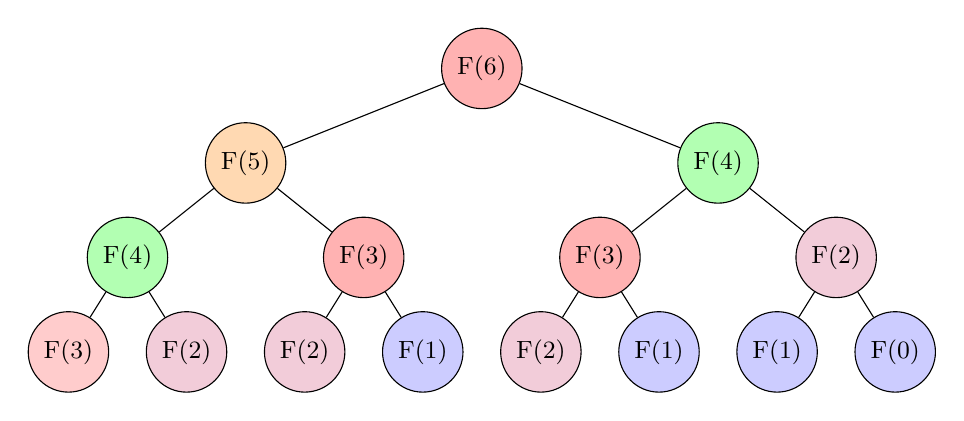
\begin{tikzpicture}[
    level distance=1.2cm,
    level 1/.style={sibling distance=6cm},
    level 2/.style={sibling distance=3cm},
    level 3/.style={sibling distance=1.5cm},
    every node/.style={circle, draw, minimum size=0.8cm, font=\small}
]
\node[fill=red!30] {F(6)}
    child {node[fill=orange!30] {F(5)}
        child {node[fill=green!30] {F(4)}
            child {node[fill=red!20] {F(3)}}
            child {node[fill=purple!20] {F(2)}}
        }
        child {node[fill=red!30] {F(3)}
            child {node[fill=purple!20] {F(2)}}
            child {node[fill=blue!20] {F(1)}}
        }
    }
    child {node[fill=green!30] {F(4)}
        child {node[fill=red!30] {F(3)}
            child {node[fill=purple!20] {F(2)}}
            child {node[fill=blue!20] {F(1)}}
        }
        child {node[fill=purple!20] {F(2)}
            child {node[fill=blue!20] {F(1)}}
            child {node[fill=blue!20] {F(0)}}
        }
    };
\end{tikzpicture}
\end{center}

\textbf{Observation :} F(3) est calculé \textcolor{importantrouge}{\textbf{3 fois}}, F(2) est calculé \textcolor{importantrouge}{\textbf{5 fois}} !
\end{exemple}

\begin{notecours}
\textbf{Points importants (notes manuscrites) :}
\begin{itemize}
    \item Équation récursif $\rightarrow$ table (remplir ligne par ligne c polynomiale avec la resultat à la dernier case en bas à gauche)
    \item Ex CC: un problème récursif $\rightarrow$ équation récursif $\rightarrow$ arbre
\end{itemize}
\end{notecours}

\subsection{Étape 3 : Algorithmes de Mémorisation et Itératif}

\begin{algorithme}
\textbf{Version avec mémorisation (top-down) :}
\begin{verbatim}
Fonction Fib(n)
Données : table[0..n] initialisée à -1
Début
    Si n $\leq$ 1 Alors
        Retourner 1
    FinSi
    
    Si table[n] $\neq$ -1 Alors
        Retourner table[n]
    FinSi
    
    table[n] ← Fib(n-1) + Fib(n-2)
    Retourner table[n]
Fin
\end{verbatim}

\textbf{Complexité :} O(n) - linéaire !
\end{algorithme}

\begin{algorithme}
\textbf{Version programmation dynamique (bottom-up, itérative) :}
\begin{verbatim}
Fonction Fib(n)
Début
    F[0] ← 1
    F[1] ← 1
    
    Pour i = 2 à n Faire
        F[i] ← F[i-1] + F[i-2]
    FinPour
    
    Retourner F[n]
Fin
\end{verbatim}

\textbf{Complexité :} O(n) linéaire, dérécursifier
\end{algorithme}

\begin{notecours}
\textbf{Notes manuscrites :}
\begin{itemize}
    \item O(n) \textbf{linéaire dérucersifier}
    \item Récursif de nature O($2^n$)
\end{itemize}
\end{notecours}

\newpage
\section{Cas d'Étude : Coefficients Binomiaux}

\subsection{Définition du Problème}

\begin{definition}
Les \textbf{coefficients binomiaux} représentent le nombre de façons de choisir k éléments parmi n éléments sans tenir compte de l'ordre.

Notation : $\binom{n}{k}$ ou C(n,k)

\textbf{Interprétation :} Nombre de parties de taille k dans un ensemble de n éléments.
\end{definition}

\begin{exemple}
\textbf{Triangle de Pascal :}

\begin{verbatim}
n=0:                    1
n=1:                  1   1
n=2:                1   2   1
n=3:              1   3   3   1
n=4:            1   4   6   4   1
n=5:          1   5  10  10   5   1
n=6:        1   6  15  20  15   6   1
\end{verbatim}
\end{exemple}

\subsection{Étape 1 : Caractérisation de la Structure}

\begin{important}
\textbf{Structure d'une solution optimale :}

Pour construire un hypercube avec n=k :
\begin{itemize}
    \item On a besoin de deux hypercubes de n=k-1
    \item On relie chaque sommet d'un hypercube au sommet correspondant de l'autre
\end{itemize}

Pour calculer $\binom{n}{k}$, on peut :
\begin{enumerate}
    \item Prendre l'élément n et choisir k-1 éléments parmi les n-1 restants : $\binom{n-1}{k-1}$
    \item Ne pas prendre l'élément n et choisir k éléments parmi les n-1 restants : $\binom{n-1}{k}$
\end{enumerate}
\end{important}

\begin{notecours}
\textbf{Notes manuscrites importantes :}
\begin{itemize}
    \item Pour construire un hyper cube avec n=k en relie deux hyper cubes de n=k-1
    \item Ex hypercube : n=3
\end{itemize}
\end{notecours}

\subsection{Étape 2 : Définition Récursive}

\begin{algorithme}
\textbf{Équation récursive :}

\[
\binom{n}{k} = \begin{cases}
1 & \text{si } k = 0 \text{ ou } k = n \\
\binom{n-1}{k-1} + \binom{n-1}{k} & \text{si } 0 < k < n
\end{cases}
\]

\textbf{Version algorithmique naïve :}
\begin{verbatim}
Fonction Binomial(n, k)
Début
    Si (k = 0 OU k = n) Alors
        Retourner 1
    Sinon
        Retourner Binomial(n-1, k-1) + Binomial(n-1, k)
    FinSi
Fin
\end{verbatim}
\end{algorithme}

\subsection{Arbre d'Exécution}

\begin{exemple}
\textbf{Arbre d'exécution pour $\binom{5}{2}$ :}

\begin{center}
\begin{tikzpicture}[
    level distance=1.5cm,
    level 1/.style={sibling distance=5cm},
    level 2/.style={sibling distance=2.5cm},
    level 3/.style={sibling distance=1.5cm},
    every node/.style={draw, minimum size=1cm, font=\footnotesize}
]
\node {$\binom{5}{2}$}
    child {node {$\binom{4}{1}$}
        child {node {$\binom{3}{0}$}}
        child {node {$\binom{3}{1}$}}
    }
    child {node {$\binom{4}{2}$}
        child {node {$\binom{3}{1}$}}
        child {node {$\binom{3}{2}$}}
    };
\end{tikzpicture}
\end{center}

\textbf{Observation :} $\binom{3}{1}$ est calculé \textcolor{importantrouge}{\textbf{2 fois}} !
\end{exemple}

\subsection{Étape 3 : Algorithme de Programmation Dynamique}

\begin{algorithme}
\textbf{Version programmation dynamique (remplissage du triangle) :}
\begin{verbatim}
Algorithme Binomial(n, k)
Données : n, k : entier
Résultat : entier
Début
    // Initialisation
    Pour i = 0 à n Faire
        Binomial[i, 0] ← 1
        Binomial[i, i] ← 1
    FinPour
    
    // Remplissage du tableau
    Pour i = 2 à n Faire
        Pour j = 1 à min(i, k) Faire
            Si (j = 0 OU j = i) Alors
                Binomial[i, j] ← 1
            Sinon
                Binomial[i, j] ← Binomial[i-1, j-1] 
                                + Binomial[i-1, j]
            FinSi
        FinPour
    FinPour
    
    Retourner Binomial[n, k]
Fin
\end{verbatim}

\textbf{Complexité :} O(n $\cdot$ k)
\end{algorithme}

\begin{notecours}
\textbf{Note importante (manuscrite) :}

L'algorithme rempli la moitié du tableau de côté n et k, donc la complexité temporelle est de l'ordre de k.n.
\end{notecours}

\begin{exemple}
\textbf{Tableau rempli pour n=6, k=6 :}

\begin{center}
\begin{tabular}{c|ccccccc}
n \textbackslash k & 0 & 1 & 2 & 3 & 4 & 5 & 6 \\
\hline
0 & 1 & & & & & & \\
1 & 1 & 1 & & & & & \\
2 & 1 & 2 & 1 & & & & \\
3 & 1 & 3 & 3 & 1 & & & \\
4 & 1 & 4 & 6 & 4 & 1 & & \\
5 & 1 & 5 & 10 & 10 & 5 & 1 & \\
6 & 1 & 6 & 15 & 20 & 15 & 6 & 1 \\
\end{tabular}
\end{center}
\end{exemple}

\newpage
\section{Aperçu : Plus Court Chemin (Floyd-Warshall)}

\begin{notecours}
\textbf{Note importante du cours :}

L'algorithme de Floyd-Warshall \textbf{ne va pas être abordé en détail} cette année pour le contrôle. Voici juste un aperçu du principe.
\end{notecours}

\subsection{Problème}

\begin{definition}
\textbf{Problème du plus court chemin pour toutes les paires :}

Soit un graphe G=(S,A) orienté valué. Pour chaque couple de sommets (s$_i$, s$_j$), déterminer le plus court chemin, s'il existe, qui joint s$_i$ à s$_j$.
\end{definition}

\subsection{Étape 1 : Structure d'une Solution Optimale}

\begin{important}
\textbf{Principe :}

Si f est un chemin de longueur minimale joignant x à y et qui passe par z, alors il se décompose en deux chemins de longueur minimale :
\begin{itemize}
    \item Le premier joint x à z
    \item Le second joint z à y
\end{itemize}
\end{important}

\subsection{Étape 2 : Définition Récursive}

\begin{algorithme}
\textbf{Équation récursive :}

Pour tout k > 0, on note $\delta_k(s_i, s_j)$ la longueur du plus court chemin de $s_i$ à $s_j$ utilisant uniquement des sommets intermédiaires d'indice < k.

\[
\delta_1(s_i, s_j) = l(s_i, s_j) \text{ ou } \infty
\]

\[
\delta_{k+1}(s_i, s_j) = \min[\delta_k(s_i, s_j), \delta_k(s_i, s_k) + \delta_k(s_k, s_j)]
\]
\end{algorithme}

\begin{notecours}
\textbf{Observation manuscrite :}

CC: équation récursif $\rightarrow$ Lda récursif
\end{notecours}

\newpage
\section{Synthèse et Conseils pour le Contrôle}

\subsection{Points Essentiels à Retenir}

\begin{important}
\textbf{Pour le contrôle, vous devez savoir :}

\begin{enumerate}
    \item \textbf{Étape 1 - Caractérisation :}
    \begin{itemize}
        \item Identifier comment une solution se décompose en sous-problèmes
        \item Expliquer la structure récursive du problème
        \item Montrer que la solution optimale contient des solutions optimales de sous-problèmes
    \end{itemize}
    
    \item \textbf{Étape 2 - Définition récursive :}
    \begin{itemize}
        \item Écrire l'équation récursive
        \item Identifier les cas de base
        \item Identifier les cas récursifs
    \end{itemize}
\end{enumerate}

\textbf{Vous n'avez PAS besoin de :}
\begin{itemize}
    \item Écrire l'algorithme complet de programmation dynamique (étape 3)
    \item Reconstruire la solution effective (étape 4)
\end{itemize}
\end{important}

\subsection{Principe d'Optimalité de Bellman}

\begin{definition}
\textbf{Rappel crucial :}

Un problème possède la propriété de sous-structure optimale si une solution optimale contient la solution optimale des sous-problèmes.

\textcolor{importantrouge}{\textbf{Toute solution optimale s'appuie elle-même sur des sous-problèmes résolus localement de façon optimale.}}
\end{definition}

\subsection{Comparaison des Approches}

\begin{center}
\colorbox{fondbleu}{
\begin{tabular}{|l|c|c|}
\hline
\rowcolor{titrebleu!30}
\textbf{Approche} & \textbf{Fibonacci} & \textbf{Binomiaux} \\
\hline
Récursif naïf & O($2^n$) & O($2^n$) \\
\hline
Mémorisation (top-down) & O(n) & O(n $\cdot$ k) \\
\hline
\rowcolor{defvert!20}
Prog. Dynamique (bottom-up) & \textcolor{defvert}{O(n)} & \textcolor{defvert}{O(n $\cdot$ k)} \\
\hline
\end{tabular}}
\end{center}

\subsection{Méthodologie pour le Contrôle}

\begin{algorithme}
\textbf{Comment aborder un problème :}

\begin{enumerate}
    \item \textbf{Lire attentivement} l'énoncé
    
    \item \textbf{Identifier} la structure récursive :
    \begin{itemize}
        \item Comment le problème se décompose-t-il ?
        \item Quels sont les sous-problèmes ?
    \end{itemize}
    
    \item \textbf{Caractériser} (Étape 1) :
    \begin{itemize}
        \item Expliquer en français comment une solution optimale se construit
        \item Montrer que les sous-problèmes sont aussi optimaux
    \end{itemize}
    
    \item \textbf{Définir récursivement} (Étape 2) :
    \begin{itemize}
        \item Écrire les cas de base
        \item Écrire la relation de récurrence
        \item Utiliser une notation mathématique claire
    \end{itemize}
\end{enumerate}
\end{algorithme}

\begin{notecours}
\textbf{Derniers conseils (notes manuscrites) :}
\begin{itemize}
    \item \textbf{Rappeler que ce que un dictionnaire, implémenter cette structure avec un tas}
    \item Le prof a donné des éléments d'examen : le chapitre 1 et chapitre 2 TDA + DÉFINITION
    \item Union find : spécification, gestion de partiotion aussi, test d'arrêt (numérique ou comme en Td)
\end{itemize}
\end{notecours}

\subsection{Applications de la Programmation Dynamique}

\begin{exemple}
\textbf{Domaines d'application :}

\begin{itemize}
    \item \textbf{Plus grande sous-séquence commune} (LCS problem)
    \item \textbf{Plus longue sous-séquence croissante}
    \item \textbf{Sac à dos} (Knapsack problem)
    \item \textbf{Plus court chemin} (Floyd-Warshall, Bellman-Ford)
    \item \textbf{Alignement de séquences} (bioinformatique)
    \item \textbf{Optimisation de chaînes de matrices}
    \item Et bien d'autres...
\end{itemize}
\end{exemple}

\newpage
\section{Conclusion}

\begin{important}
La programmation dynamique est un paradigme puissant qui permet de résoudre efficacement des problèmes d'optimisation en évitant de recalculer plusieurs fois les mêmes sous-problèmes.

\textbf{Les points essentiels :}
\begin{itemize}
    \item \textcolor{titrebleu}{Principe d'optimalité de Bellman} : solution optimale = composition de solutions optimales de sous-problèmes
    
    \item \textcolor{titrebleu}{Différence avec diviser pour régner} : sous-problèmes interdépendants vs indépendants
    
    \item \textcolor{titrebleu}{Processus en 4 étapes} : caractériser, définir, calculer, reconstruire
    
    \item \textcolor{titrebleu}{Pour le contrôle} : maîtriser les 2 premières étapes
\end{itemize}
\end{important}

\begin{notecours}
\textbf{Récapitulatif final :}
\begin{itemize}
    \item Se base sur des calcules exactes
    \item C'est un paradigme pour résoudre des problèmes
    \item Adaptation de "diviser pour régner" quand les sous-problèmes ne sont pas indépendants
    \item Équation récursif $\rightarrow$ arbre $\rightarrow$ table (polynomiale)
    \item Complexité réduite de exponentielle à polynomiale
\end{itemize}
\end{notecours}

\vspace{2em}

\begin{center}
\large\textbf{Bon courage pour le contrôle !}
\end{center}

% ============================================================
%  EXERCICE : Distance d'édition (Levenshtein) - Q1 & Q2 + arbre
% ============================================================

\newpage
\section{Exemple (CC) : Distance d'édition entre deux mots}

\subsection{Énoncé}
On considère deux mots $s[1..n]$ et $t[1..m]$.
La \textbf{distance d'édition} (ou distance de Levenshtein) est le \textbf{nombre minimal d'opérations} permettant de transformer $s$ en $t$ en utilisant :
\begin{itemize}
    \item \textbf{insertion} (coût 1),
    \item \textbf{suppression} (coût 1),
    \item \textbf{substitution} (coût 1).
\end{itemize}

\begin{important}
\textbf{Pour le contrôle :} on demande ici uniquement \textcolor{importantrouge}{\textbf{(1) l'équation récursive}} et \textcolor{importantrouge}{\textbf{(2) l'algorithme récursif naïf (LDA)}}, ainsi que l'arbre d'appels sur un exemple.
\end{important}

\subsection{Notations}
On note
\[
dist(s,t,i,j)
\]
la distance d'édition entre les \textbf{préfixes} $s[1..i]$ et $t[1..j]$.

\begin{definition}
\[
dist(s,t,i,j) = \text{nombre minimal d'opérations (insertion/suppression/substitution) pour transformer } s[1..i] \text{ en } t[1..j].
\]
\end{definition}

% ------------------------------------------------------------
% Q1 : Définition récursive
% ------------------------------------------------------------
\subsection{(1) Définition récursive de $dist(s,t,i,j)$}

\begin{algorithme}
\textbf{Cas de base :}
\[
dist(s,t,0,j)=j \qquad\text{(il faut insérer les $j$ caractères de $t[1..j]$)}
\]
\[
dist(s,t,i,0)=i \qquad\text{(il faut supprimer les $i$ caractères de $s[1..i]$)}
\]

\medskip
\textbf{Cas récursif :} pour $i>0$ et $j>0$,
\[
dist(s,t,i,j)=
\begin{cases}
dist(s,t,i-1,j-1) & \text{si } s[i]=t[j],\\[0.4em]
1+\min\big(dist(s,t,i-1,j),\,dist(s,t,i,j-1),\,dist(s,t,i-1,j-1)\big) & \text{si } s[i]\neq t[j].
\end{cases}
\]

\medskip
\textbf{Interprétation des 3 termes du minimum (si $s[i]\neq t[j]$) :}
\begin{itemize}
    \item $dist(s,t,i-1,j)+1$ : \textbf{suppression} de $s[i]$,
    \item $dist(s,t,i,j-1)+1$ : \textbf{insertion} de $t[j]$,
    \item $dist(s,t,i-1,j-1)+1$ : \textbf{substitution} de $s[i]$ par $t[j]$.
\end{itemize}
\end{algorithme}

\begin{notecours}
\textbf{Pourquoi $dist(i-1,j-1)$ apparaît deux fois ?}
\begin{itemize}
    \item Si $s[i]=t[j]$ : on \textbf{ne paie rien} (pas d'opération) $\Rightarrow dist(i-1,j-1)$.
    \item Si $s[i]\neq t[j]$ : on peut choisir la \textbf{substitution} (coût 1) $\Rightarrow 1+dist(i-1,j-1)$.
\end{itemize}
\end{notecours}

% ------------------------------------------------------------
% Q2 : Algorithme récursif naïf (LDA)
% ------------------------------------------------------------
\subsection{(2) Algorithme récursif naïf (LDA)}

\begin{algorithme}
\textbf{Algorithme $dist$ (récursif naïf) :}
\begin{verbatim}
Fonction dist(s, t, i, j)
Début
    Si i = 0 Alors
        Retourner j
    FinSi
    Si j = 0 Alors
        Retourner i
    FinSi

    Si s[i] = t[j] Alors
        Retourner dist(s, t, i-1, j-1)
    Sinon
        Retourner 1 + min(
            dist(s, t, i-1, j),     // suppression
            dist(s, t, i, j-1),     // insertion
            dist(s, t, i-1, j-1)    // substitution
        )
    FinSi
Fin
\end{verbatim}

\textbf{Remarque :} cet algorithme est correct mais \textcolor{importantrouge}{\textbf{recalcule}} plusieurs fois les mêmes sous-problèmes.
\end{algorithme}

% ------------------------------------------------------------
% Exemple + arbre d'appels
% ------------------------------------------------------------
\subsection{Exemple : $s=\texttt{lou}$ et $t=\texttt{ole}$}

\begin{exemple}
On indexe :
\[
s=\texttt{lou}\ (n=3),\quad t=\texttt{ole}\ (m=3)
\]
\[
s[1]=l,\ s[2]=o,\ s[3]=u \qquad t[1]=o,\ t[2]=l,\ t[3]=e
\]

On cherche $dist(s,t,3,3)$. Le résultat obtenu est :
\[
dist(\texttt{lou},\texttt{ole},3,3)=3.
\]
\end{exemple}

\subsection{Arbre d'appels récursifs (extrait)}
\begin{exemple}
\textbf{Arbre (premiers niveaux) pour $dist(3,3)$ :}

\begin{center}
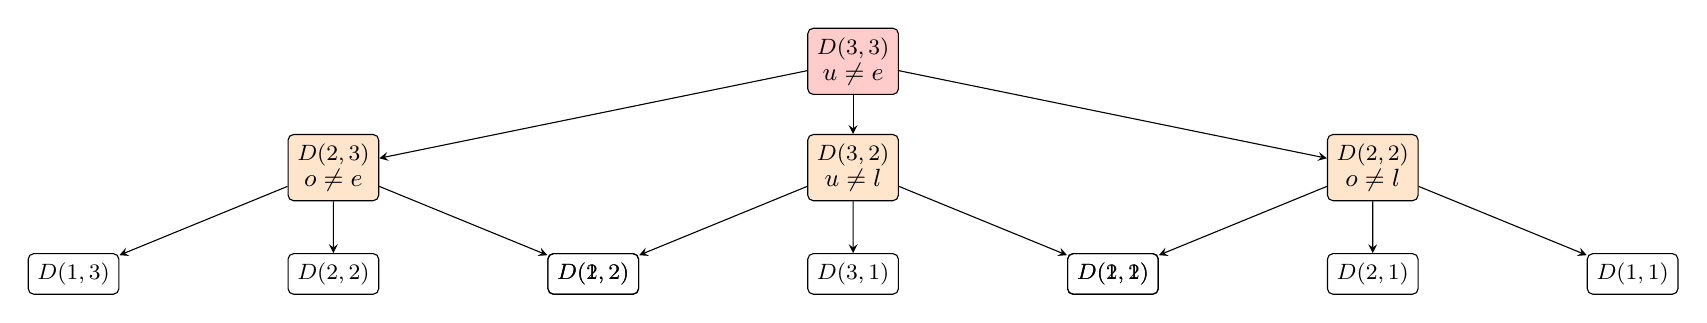
\begin{tikzpicture}[
    level distance=1.35cm,
    level 1/.style={sibling distance=6.6cm},
    level 2/.style={sibling distance=3.3cm},
    level 3/.style={sibling distance=1.8cm},
    every node/.style={draw, rounded corners=2pt, align=center, font=\footnotesize},
    edge from parent/.style={-stealth, draw}
]
\node[fill=red!20] {$D(3,3)$\\ \small $u\neq e$}
    child { node[fill=orange!20] {$D(2,3)$\\ \small $o\neq e$}
        child { node {$D(1,3)$} }
        child { node {$D(2,2)$} }
        child { node {$D(1,2)$} }
    }
    child { node[fill=orange!20] {$D(3,2)$\\ \small $u\neq l$}
        child { node {$D(2,2)$} }
        child { node {$D(3,1)$} }
        child { node {$D(2,1)$} }
    }
    child { node[fill=orange!20] {$D(2,2)$\\ \small $o\neq l$}
        child { node {$D(1,2)$} }
        child { node {$D(2,1)$} }
        child { node {$D(1,1)$} }
    };
\end{tikzpicture}
\end{center}

\textbf{Observation :} le sous-problème \textcolor{importantrouge}{\textbf{$D(2,2)$}} apparaît \textcolor{importantrouge}{\textbf{plusieurs fois}} $\Rightarrow$ recalculs $\Rightarrow$ motivation de la programmation dynamique.
\end{exemple}

\begin{notecours}
\textbf{Point méthode (contrôle) :}
\begin{itemize}
    \item Étape 1 (structure) : on compare des \textbf{préfixes} et on enlève 1 caractère à gauche/droite.
    \item Étape 2 (récurrence) : cas de base $i=0$ / $j=0$ puis min des 3 opérations.
    \item L'arbre montre que l'approche récursive naïve explose (beaucoup de répétitions).
\end{itemize}
\end{notecours}
\end{document}